\section{Background}\label{sec:lr_background}
\noindent \textbf{Steiner trees.} A multicast tree carries one copy of a stream from a source to many receivers, duplicating packets only where paths split. Finding the minimum-cost such tree is the Steiner tree problem in graphs, which is NP-hard, so practical systems use polynomial heuristics. The two standard references are \textbf{MPH}~\cite{takahashi1980mph}, which grows the tree from the source by repeatedly attaching the nearest unconnected terminal through its shortest path, and \textbf{KMB}~\cite{kou1981kmb}, which builds a minimum spanning tree on the terminals' distance graph, expands it into shortest paths and prunes it. Both guarantee a single-rate tree at most $2(1-1/l)$ times optimal for $l$ leaves.

\noindent \textbf{Multi-rate trees.} When receivers request different qualities, a link must carry the highest rate needed below it. Building a Steiner tree for the highest layer first and extending it layer by layer (the ``top-down'' heuristic) is within $\frac{\ell+1}{2}\rho$ of optimal for $\ell$ nested layers, where $\rho$ is the ratio of the Steiner heuristic used~\cite{ahmed2019mlst}; dedicated algorithms for arbitrary rates reach $e\cdot\rho$~\cite{charikar2004qos}. The layered MPH used in this thesis is the top-down heuristic with MPH as the Steiner step.

\noindent \textbf{Multi-rate delivery.} Receiver-driven layered multicast~\cite{mccanne1996rlm} sends cumulative video layers on separate multicast groups, so each receiver subscribes up to its own rate and a shared link carries the highest layer needed below it. The thesis adopts this delivery model.

\noindent \textbf{SDN.} Software-defined networking separates the control plane from the switches: a central controller with a global view computes trees and installs per-switch OpenFlow rules. This makes centralised, learned and repairable multicast routing practical, but every tree change costs rule updates at the switches.

\section{Key Related Research}\label{sec:lr_related}
\noindent \textbf{Wang \emph{et al.}}~\cite{wang2026gnn} (the base paper) formulate multi-quality multicast as a constrained minimum-flow problem and prove that the optimal flow-carrying links form a source-rooted tree in which a shared link carries the maximum demand of the receivers below it (Lemma~1, Figure~\ref{fig:bp_example}). Their graph policy network (GPN, Figure~\ref{fig:gpn_arch}) combines a GAT encoder (hidden size 128, 4 heads), an LSTM path-history aggregator and an attention pointer decoder, with under 3\,M parameters, trained by policy gradient on 30-node Erd\H{o}s--R\'enyi graphs with 9 users. Users are routed in descending demand order, and each path grows hop by hop until it touches the existing tree, so branches are reused (Figure~\ref{fig:bp_sequential}). On 30--50-node random graphs GPN beats shortest-path and plain-GAT routing, matches bee-colony optimization and stays slightly above GA and the DP optimum while running orders of magnitude faster (Figure~\ref{fig:bp_results}). Its limitation is that the tree is built once for a fixed audience: the only dynamic test adds 1--3 users, and leaves, quality changes, link failures, capacity and rule-change cost are not modelled.

\begin{figure}[!htb]
\centering
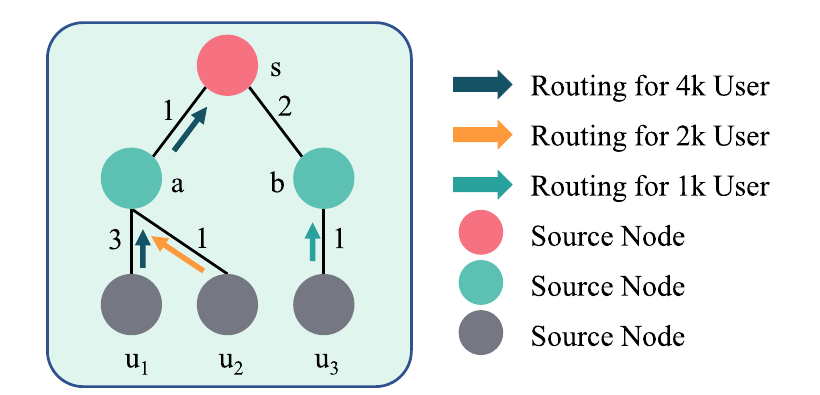
\includegraphics[width=0.5\textwidth]{fig2.png}
\caption[Routing example of the base paper (Lemma 1)]{A shared link carries the highest downstream demand (Lemma~1)~\cite{wang2026gnn}.}
\label{fig:bp_example}
\end{figure}

\begin{figure}[!htb]
\centering
\begin{tikzpicture}[
    font=\small,
    box/.style={draw, rounded corners=3pt, align=center, minimum height=1.2cm, text width=2.6cm, fill=white},
    acc/.style={box, draw=blue!70!black, fill=blue!6, thick},
    arr/.style={-{Stealth[length=2.2mm]}, thick, gray!70!black},
    lab/.style={font=\scriptsize, text=gray!40!black, align=center}]
  \node[box] (in) {Graph $G=(V,E)$,\\link costs,\\user demands};
  \node[acc, right=0.85cm of in] (gat) {GAT encoder\\$H=128$, 4 heads};
  \node[box, right=0.85cm of gat] (lstm) {LSTM path-\\history aggregator};
  \node[acc, right=0.85cm of lstm] (dec) {Attention\\pointer decoder};
  \node[box, below=1.0cm of dec] (act) {Next hop $v_t$\\(softmax over\\unvisited nodes)};
  \node[draw, dashed, rounded corners=3pt, align=left, font=\footnotesize, text width=6.4cm, anchor=north west] (rew) at ($(in.south west)+(0,-0.8)$) {Trained by policy gradient with per-step reward $r_t=-x_{(k)}\,e(u_t,v_t)$. A path grows until it reaches the existing tree; then the next user (in descending demand order) is routed.};
  \draw[arr] (in) -- (gat);
  \draw[arr] (gat) -- (lstm);
  \draw[arr] (lstm) -- node[above, lab] {$h_t$} (dec);
  \draw[arr] (gat.north) to[bend left=18] node[above, lab] {node embeddings of candidate next hops} (dec.north);
  \draw[arr] (dec) -- (act);
  \draw[arr] (act.west) -| node[right, lab, pos=0.75] {selected node\\fed back} (lstm.south);
\end{tikzpicture}
\caption[Architecture of the base paper's graph policy network (GPN)]{Architecture of the base paper's GPN~\cite{wang2026gnn}.}
\label{fig:gpn_arch}
\end{figure}

\begin{figure}[!htb]
\centering
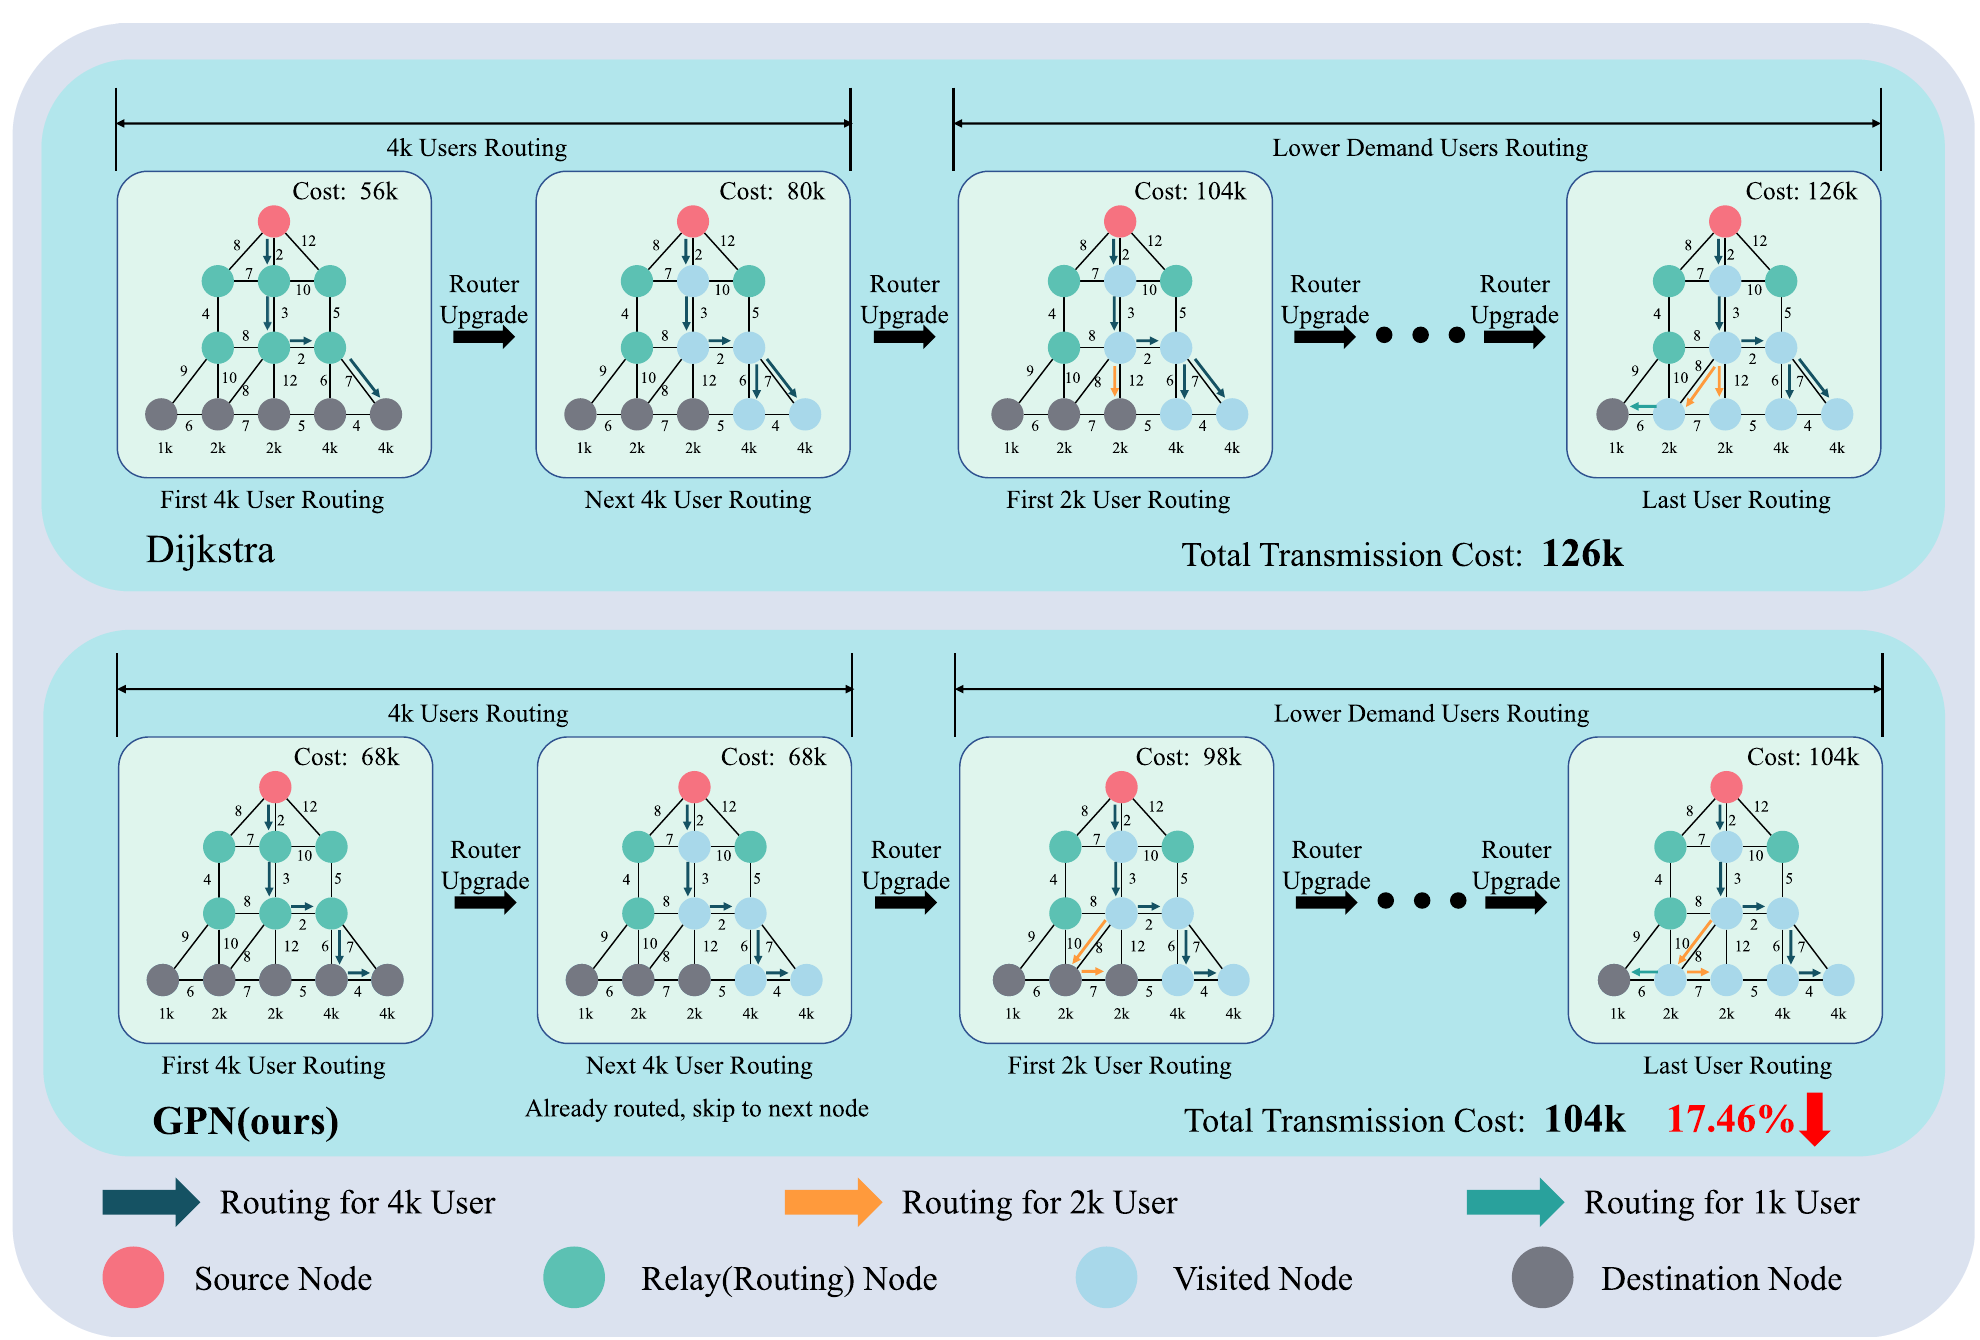
\includegraphics[width=0.92\textwidth]{fig1.png}
\caption[Sequential routing in the base paper: Dijkstra vs.\ GPN]{Routing under sequential user arrivals: Dijkstra (top) builds independent paths, while GPN (bottom) reuses branches and cuts total cost by 17.46\% in this example~\cite{wang2026gnn}.}
\label{fig:bp_sequential}
\end{figure}

\begin{figure}[!htb]
\centering
\begin{minipage}[t]{0.48\textwidth}\centering
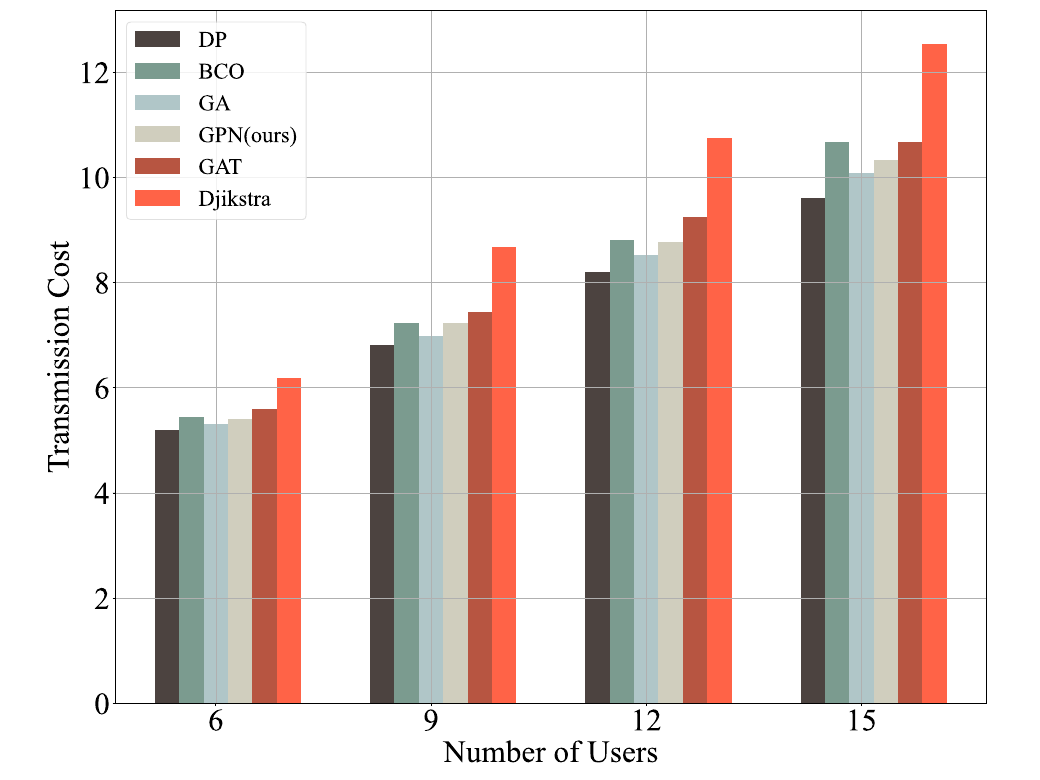
\includegraphics[width=\textwidth]{fig7.png}\\[-2pt]{\small (a) Cost vs.\ users (6--15), 50 nodes}
\end{minipage}\hfill
\begin{minipage}[t]{0.48\textwidth}\centering
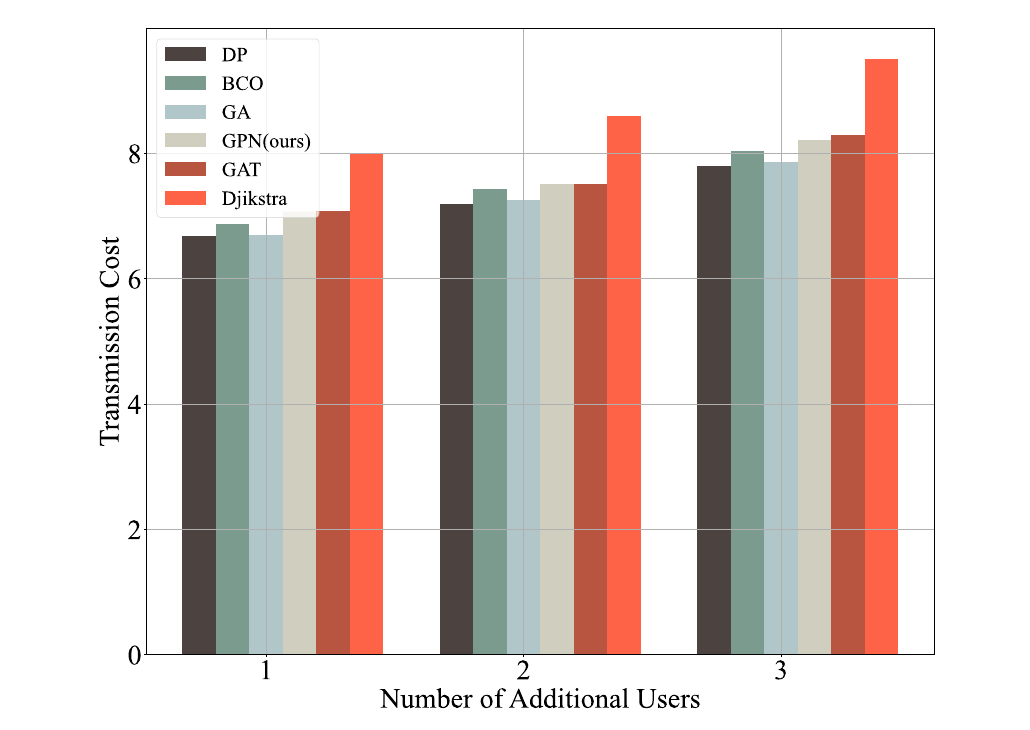
\includegraphics[width=\textwidth]{fig13.png}\\[-2pt]{\small (b) Cost after adding 1--3 users to 9}
\end{minipage}
\caption[Base paper results: cost vs.\ users and the dynamic-addition test]{Base paper results on 50-node graphs: (a) routing cost vs.\ number of users; (b) its only dynamic test~\cite{wang2026gnn}.}
\label{fig:bp_results}
\end{figure}

\noindent \textbf{Zhao \emph{et al.}}~\cite{zhao2022drlm4mr} proposed DRL-M4MR, which treats the network as four $n\times n$ matrices (tree state, residual bandwidth, delay, loss) and uses a double dueling DQN with prioritised replay to add one link per step. In Ryu/Mininet on a 14-node topology it raised bottleneck bandwidth by 19.37\% over KMB. Its limitation is that its trees used 15--30\% more links, its fixed-size matrix input ties the model to one topology, and it re-solves for a fixed destination set.

\noindent \textbf{Zhang \emph{et al.}}~\cite{zhang2026ghacmr} proposed GHAC-MR, which uses graph message passing with a PPO actor--critic and Bernoulli per-link forwarding actions, and reports lower delay and loss than KMB, GA, DRL-M4MR and a hierarchical-RL router on three topologies. Its limitation is that it also rebuilds trees for a fixed destination set without modelling leaves, quality changes or rule churn, and its own results show the hierarchical-RL router with higher bandwidth on Fat-Tree (16.74 vs.\ 14.63).

\noindent \textbf{Imase and Waxman}~\cite{imase1991dynamic} studied the dynamic Steiner tree problem and showed that a greedy online tree is $O(\log n)$-competitive as receivers join, and that a limited number of rearrangements restores a constant-factor bound when receivers also leave. This is the cost-versus-rearrangement trade-off that this thesis measures when comparing local repair with full re-planning. Its limitation is that the analysis assumes a single rate and no link capacities, and gives no learned or practical policy for when to rearrange.

\noindent \textbf{Shen \emph{et al.}}~\cite{shen2015rst} proposed the Recover-aware Steiner Tree (RST) for SDN multicast, which jointly minimises tree cost and the cost of recovering from link failures, and validated it on an SDN testbed. Its limitation is that it handles a single rate and a fixed group, and does not consider receiver churn or the cost of reconfiguring switch rules.

\noindent \textbf{Oostenbrink \emph{et al.}}~\cite{oostenbrink2017failover} pre-install backup paths as OpenFlow fast-failover groups, so switches reroute multicast traffic locally without the controller and recover in under 10\,ms. Its limitation is the extra switch memory for backup state, and the trees it protects are classical single-rate trees rather than learned multi-rate ones.

\noindent \textbf{Reitblatt \emph{et al.}}~\cite{reitblatt2012update} introduced two-phase, versioned rule updates that guarantee each packet is processed by either the old or the new configuration, never a mix. Its limitation, for this thesis, is that it makes a change safe but not cheap: it does not decide which tree to install or how many rules to change.

\noindent Table~\ref{tab:comparison} compares these works with this thesis.

\begin{table}[!htb]
\caption{Comparison of the related works}
\label{tab:comparison}
\begin{center}
\footnotesize
\renewcommand{\arraystretch}{1.1}
\begin{tabular}{|L{2.3cm}|L{2.4cm}|C{1.2cm}|L{1.8cm}|L{1.8cm}|L{1.9cm}|L{2.1cm}|}
\hline
\textbf{Work} & \textbf{Tree builder} & \textbf{Multi-rate} & \textbf{Leave / quality change} & \textbf{Link failure} & \textbf{Rule-change cost} & \textbf{Validation} \\
\hline\hline
MPH / KMB~\cite{takahashi1980mph,kou1981kmb} & Heuristic, $2(1-1/l)$ bound & No & Full re-plan & Full re-plan & Not measured & Analysis \\ \hline
Online Steiner~\cite{imase1991dynamic} & Greedy + rearrangement & No & Yes (theory) & No & Edge changes bounded & Analysis \\ \hline
DRL-M4MR~\cite{zhao2022drlm4mr} & Double dueling DQN & No & No & No & No & Ryu + Mininet, 14 nodes \\ \hline
GHAC-MR~\cite{zhang2026ghacmr} & GNN + PPO & No & No & No & No & Ryu + Mininet, 3 topologies \\ \hline
RST~\cite{shen2015rst} & Approximation & No & No & Yes (recovery cost) & No & SDN testbed \\ \hline
Fast-failover~\cite{oostenbrink2017failover} & Precomputed backups & No & Join/leave groups & Yes, $<$10\,ms & Switch memory & Emulation \\ \hline
Base paper~\cite{wang2026gnn} & GAT + LSTM pointer & Yes & Adds only & No & No & Simulation, $\le$50 nodes \\ \hline
\textbf{This thesis} & Base GPN + repair operators + MPH net & Yes & Yes & Yes, fast-failover & Yes ($\mu\times$ changes) & Simulation, Mininet/Ryu, 5G SA lab \\
\hline
\end{tabular}
\end{center}
\end{table}

\section{Research Gaps}\label{sec:lr_gap}
\noindent Learned multi-rate multicast has been shown to build good trees, but not to keep them cheap, stable and protected while the audience and the network change, and not at real receivers. The specific gaps found in the literature review are:
\begin{itemize}
    \item \textbf{Viewers leaving or lowering quality} are not modelled; only 1--3 additions are tested, so unused branches keep consuming bandwidth (addressed by the cost model and the repair operators).
    \item \textbf{Late high-quality joins} are under-priced, because the reward charges only newly added links and ignores upstream upgrades (addressed by the cost model).
    \item \textbf{Link failures and mobility} are never tested; the only recovery is a full re-plan (addressed by the repair operators and fast-failover protection).
    \item \textbf{Link capacity} is not constrained, so congestion is invisible to the model (addressed by the capacity-constrained formulation).
    \item \textbf{Reconfiguration cost} is ignored: there is no control plane, and a re-plan re-routes every user, so rule churn and video disruption are unmeasured (addressed by the rule-change penalty and two-phase updates).
    \item \textbf{No quality guarantee}: GPN is 6--7\% above optimum and was never compared with Steiner heuristics; our replication finds layered MPH at least as cheap on about 80\% of instances (addressed by the MPH safety net of the learned policy).
    \item \textbf{Evaluation} uses random graphs of at most 50 nodes, and ``delay'' means computation time, so there is no evidence at real switches or users (addressed by the three-tier evaluation).
\end{itemize}

\section{Problem Formulation}\label{sec:lr_rq}
\noindent The problem addressed by this thesis is:
\begin{itemize}
    \item Given an SDN transport network with link capacities, a video source with cumulative quality layers, and a stream of events (join, leave, quality change, link or switch failure), maintain a multi-rate multicast tree that minimises tree cost plus a penalty on rule changes, while keeping video disruption at receivers low.
\end{itemize}
\noindent The work answers three research questions:
\begin{itemize}
    \item Under realistic join, leave, quality-change and failure patterns, how many rule changes and how much recomputation do local repair operators save versus full re-planning, and at what tree-cost penalty?
    \item Can the base paper's GNN, extended to choose keep / local repair / full re-plan and paired with a certified MPH fallback, beat fixed-threshold policies on combined cost and churn?
    \item Do pre-installed backup paths measurably reduce video disruption at real 5G UEs, and how much extra switch state do they cost?
\end{itemize}
